\documentclass{standalone}
\usepackage{tikz}

\begin{document}
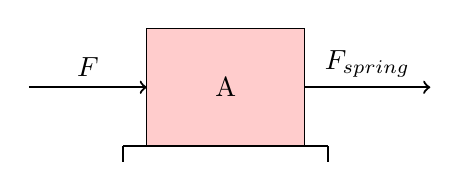
\begin{tikzpicture}

  % Cart A
  \draw[fill=red!20] (0,0) rectangle (2,1.5);
  \node at (1,0.75) {A};

  % Force F
  \draw[->, thick] (-1.5,0.75) -- (0,0.75) node[midway, above] {$F$};

  % Spring Force
  \draw[->, thick] (2,0.75) -- (3.6,0.75) node[midway, above] {\( F_{spring} \)};

  % Ground support
  \draw[thick] (-0.3,0) -- (2.3,0);
  \draw[thick] (-0.3,0) -- (-0.3,-0.2);
  \draw[thick] (2.3,0) -- (2.3,-0.2);

\end{tikzpicture}
\end{document}
